

\section{About Crop Recommendation System}
       Agriculture plays a major role in Indian economy and employment. India is one of the largest producers of agricultural products, but still it has less farm production. The most common problem faced by the farmers is that they do not opt the crop based on the necessity of soil. This problem can be solved by using crop recommendation system.\par
A crop recommendation system helps the farmers to enhance their crop production by recommending the best crops based on soil properties. This system uses machine learning algorithms to analyse the data collected from several sources. Based on this analysis,the system can  suggest the best crop to grow in a particular area,by taking the factors such as nutrient levels,temperature,rainfall,pH value,humidity etc. It helps to improve crop yields and reduce waste. It helps the farmers to save time and money in reducing the non suitable crop selection. It also helps the farmers to take better decisions for farming. This improves our Indian economy by maximizing the yield rate of crop production.
\section{Data Set}
     The dataset consists of parameters like Nitrogen(N),Phosphorus(P),
Potassium(K),pH value of the soil,Humidity,Temperature and Rainfall. The dataset have been obtained from the Kaggle website. The dataset has 2708 instance or data that have taken from the past historic data. This dataset includes nine different crops such as pomegranate,banana,
mango,grapes,watermelon,muskmelon,apple,orange and papaya.
\subsection*{Features of dataset}
N: ratio of Nitrogen content in soil\\P: ratio of Phosphorus content in soil\\K: ratio of Potassium content in soil\\Temperature: temperature in degree celsius\\Humidity: relative humidity in \%\\pH: pH value of the soil\\rainfall: rainfall in mm
\subsection*{Data Cleaning and preprocessing}
    The first step is to make sure that the dataset we are using is accurate. The dataset should not have any missing values and if the dataset have missing values,they should be replaced by appropriate values by using mean,median or mode of the entire column.
\section{Prediction techniques}
\subsection*{K-Nearest Neighbour(KNN)}
K-Nearest Neighbour is one of the simplest machine learning algorithms based on supervised learning technique.K-NN algorithm assumes the similarity between the new case and available cases and puts the new case into category that is most similar to available categories.K-NN algorithm can be used for Regression as well as for Classification but mostly it is used for the Classification problems.It is also called as a lazy learner algorithm because it does not learn from the training set immediately instead it stores the dataset and at the time of classification,it performs an action on the dataset.
\subsection*{Support Vector Machines(SVM)} 
Support Vector Machine(SVM) is one of the most popular Supervised Learning algorithms,which is used for Classification as well as Regression problems.It is used mostly for Classification problems in Machine Learning.The goal of the SVM algorithm is to create the best line or decision boundary that can segregate n-dimensional space into classes so that we can easily put the new data point in the correct category in the future.
\section{Graphs}
\subsection{Bar Graph}
\begin{lstlisting}[language=Python,basicstyle=\fontsize{9}{11}\selectfont]
x=df["label"]
y=df["rainfall"]
fig = plt.figure(figsize=(10,10))
plt.xlabel("label")
plt.ylabel("rainfall")
plt.title("Bar Graph")
plt.bar(x,y,width=0.7)
plt.show()
\end{lstlisting}
\begin{figure}[h]
\centering
 \footnotesize
 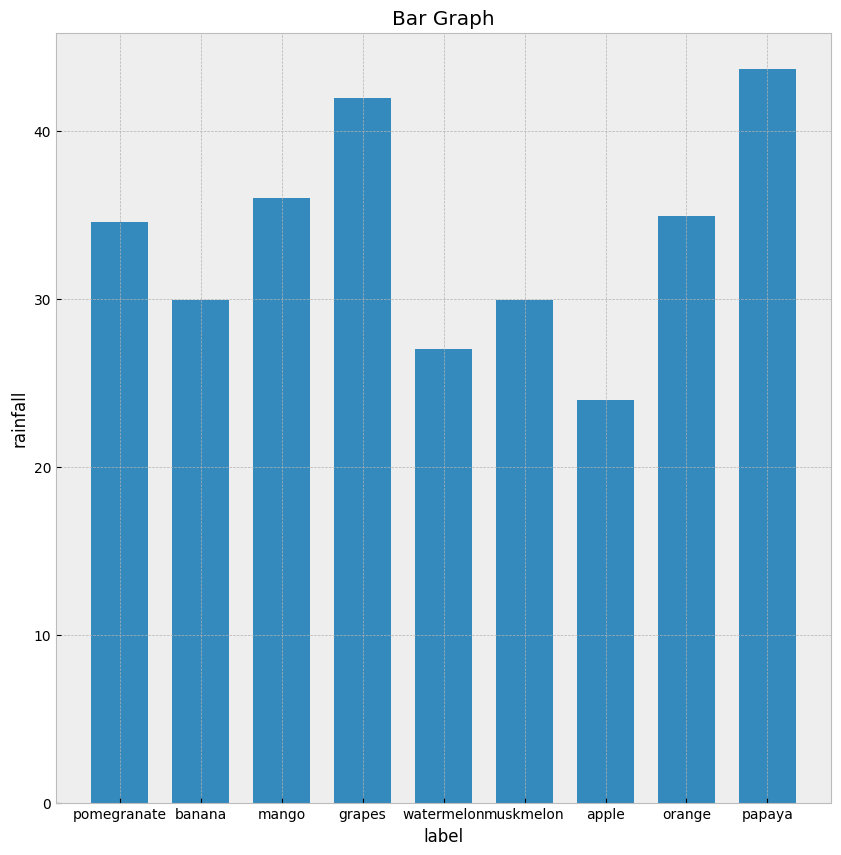
\includegraphics[width=3in,height=2in]{bar.png}
\caption{Bar Graph}
\label{fig:dunnhalftone}
\end{figure}
\subsection{Scatter Plot}
\begin{lstlisting}[language=Python,basicstyle=\fontsize{9}{11}\selectfont]
a=df["rainfall"]
b=df["humidity"]
plt.xlabel("rainfall")
plt.ylabel("humidity")
plt.title("Scatter Plot")
plt.scatter(a,b,color="green")
\end{lstlisting}
\begin{figure}[h]
\centering
 \footnotesize
 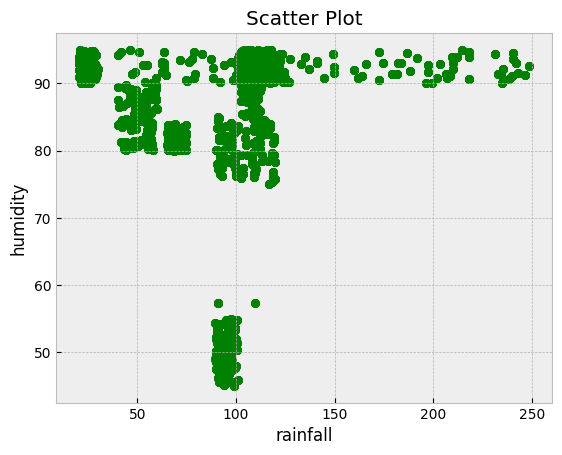
\includegraphics[width=3in,height=2in]{scatter.png}
\caption{Scatter Plot}
\label{fig:dunnhalftone}
\end{figure}
\subsection{Histogram}
\begin{lstlisting}[language=Python,basicstyle=\fontsize{9}{11}\selectfont]
plt.xlabel("temperature")
plt.title("Histogram")
df["temperature"].plot(kind="hist")
\end{lstlisting}
\begin{figure}[h]
\centering
 \footnotesize
 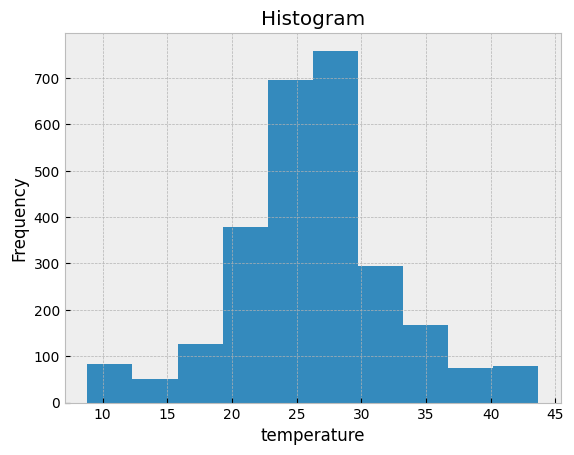
\includegraphics[width=3in,height=2in]{histogram.png}
\caption{Histogram}
\label{fig:dunnhalftone}
\end{figure}
\subsection{Box Plot}
\begin{lstlisting}[language=Python,basicstyle=\fontsize{9}{11}\selectfont]
x=df["N"]
plt.xlabel("N")
plt.title("Box Plot")
plt.boxplot(x,notch=True,patch_artist=True)
\end{lstlisting}
\begin{figure}[h]
\centering
 \footnotesize
 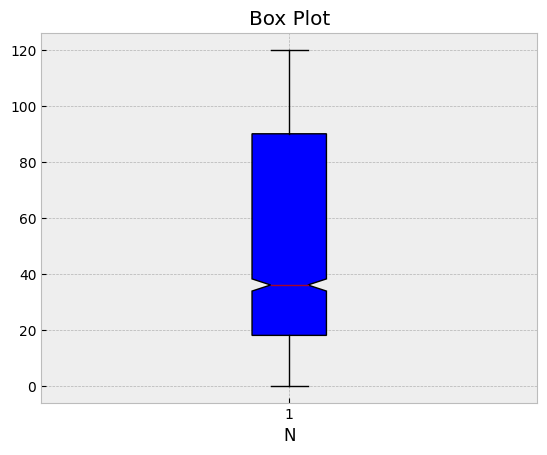
\includegraphics[width=3in,height=2in]{box.png}
\caption{Box Plot}
\label{fig:dunnhalftone}
\end{figure}
\section{Visualization}
\subsection{Pair Plot}
\begin{lstlisting}[language=Python,basicstyle=\fontsize{9}{11}\selectfont]
import seaborn as sns
sns.pairplot(df)
\end{lstlisting}
 
\begin{figure}[h]
\centering
 \footnotesize
 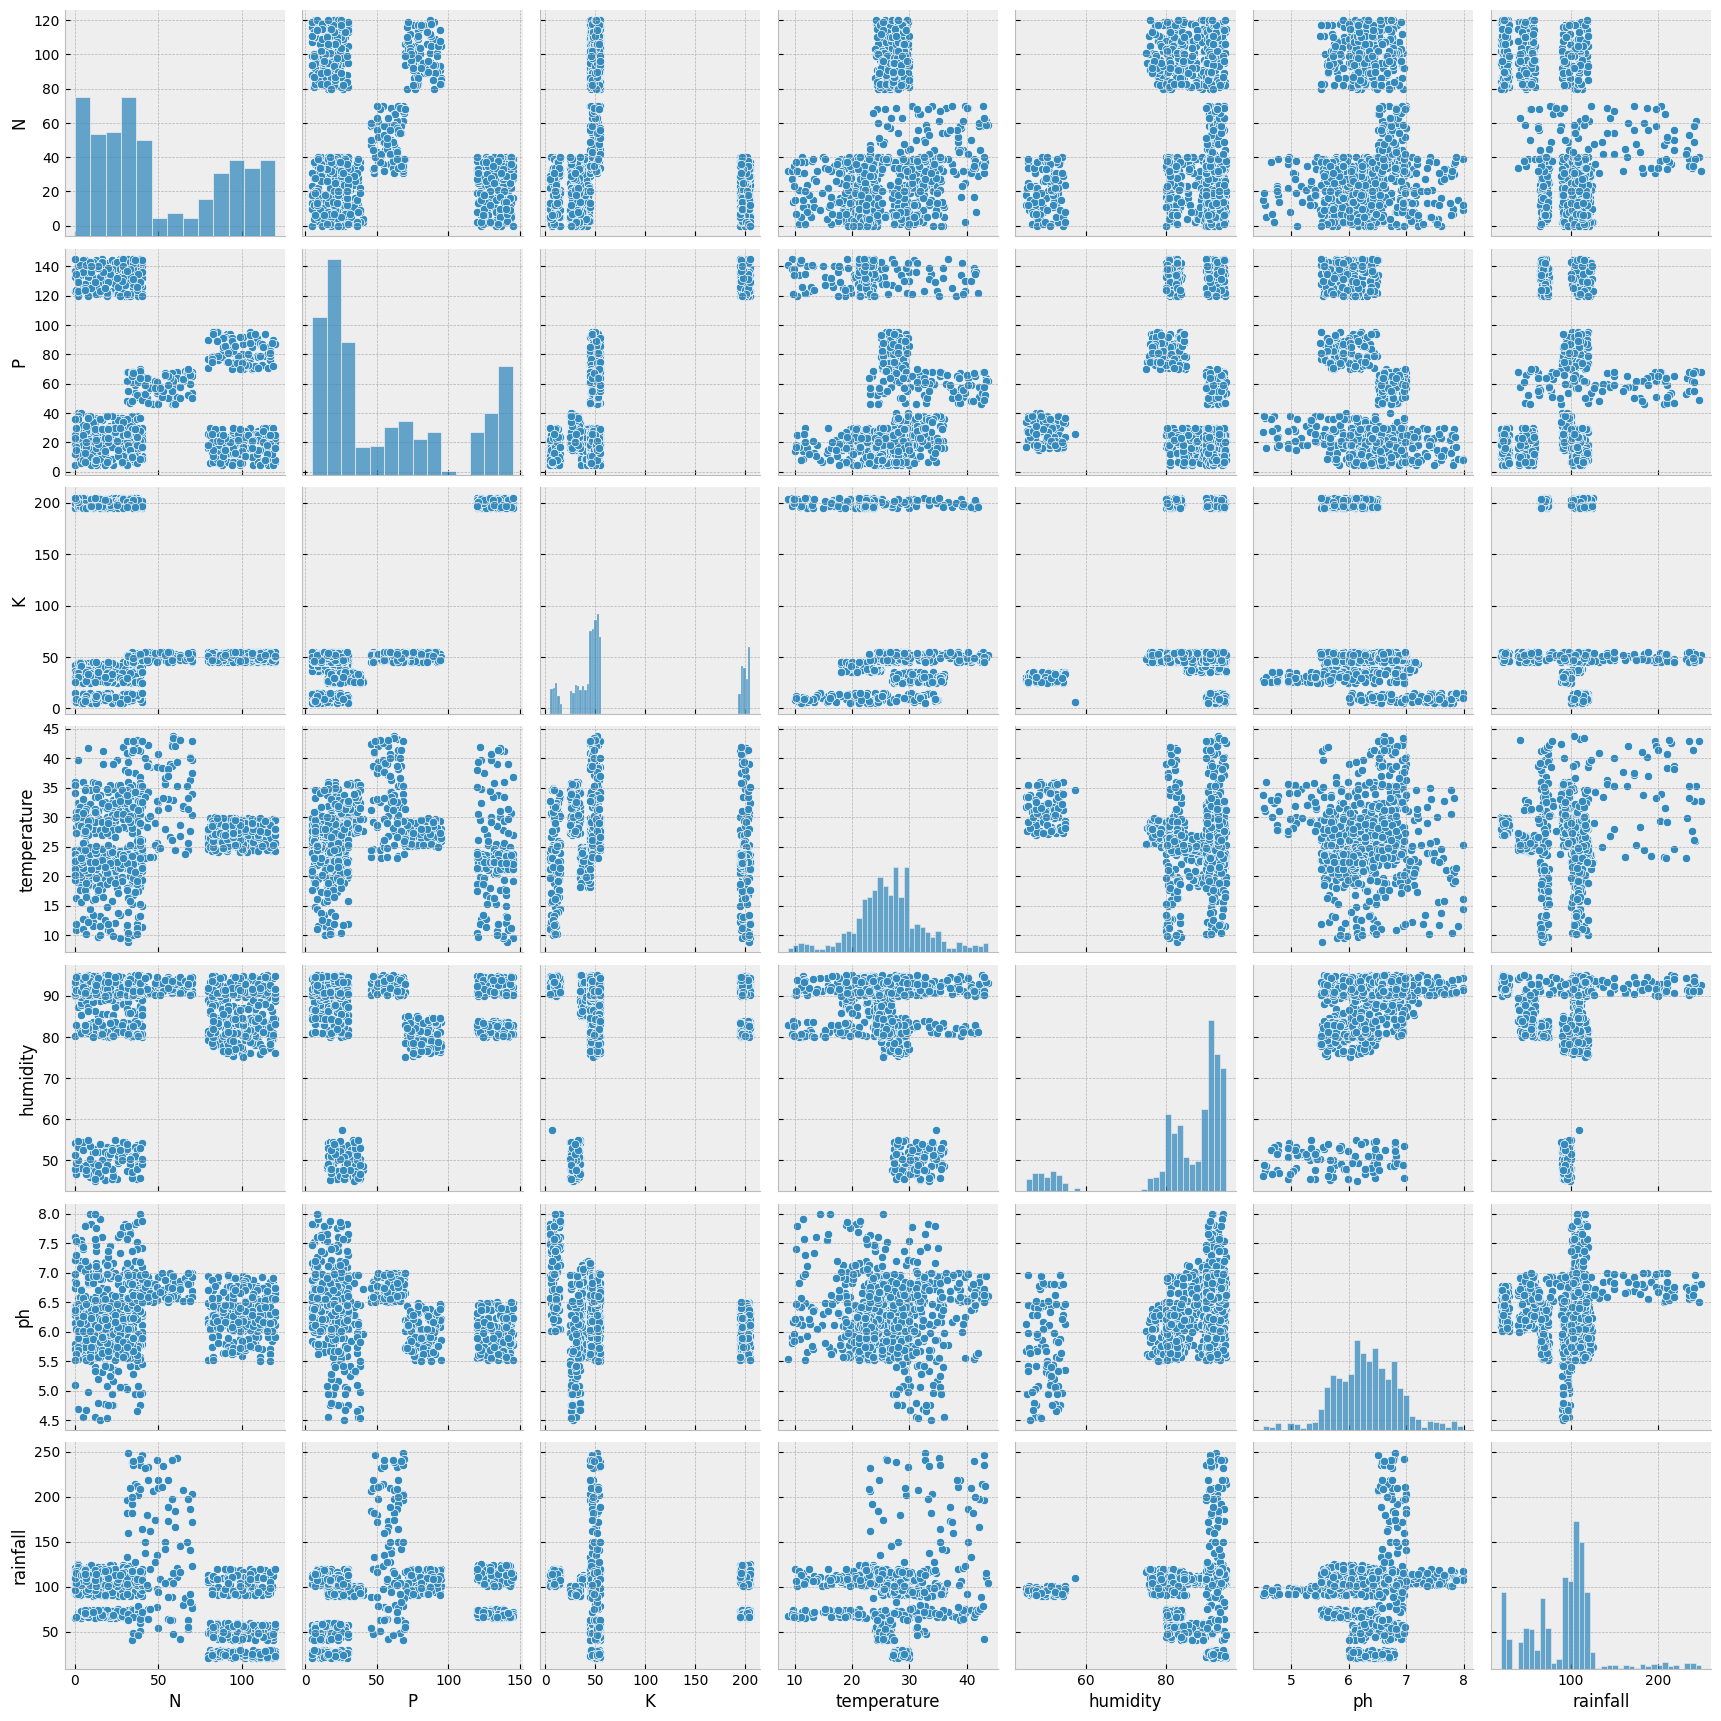
\includegraphics[width=4in,height=2in]{pair.png}
\caption{Pair Plot}
\label{fig:unevenlight}
\end{figure} 
\subsection{Bar Graph}
\begin{lstlisting}[language=Python,basicstyle=\fontsize{9}{11}\selectfont]
fig=plt.figure(figsize=(10,6))
ax=fig.add_axes([0,0,1,1])
sns.barplot(x="label",y="rainfall",data=df)
plt.title("graph showing the average rainfall for each label")
\end{lstlisting}
 
\begin{figure}[h]
\centering
 \footnotesize
 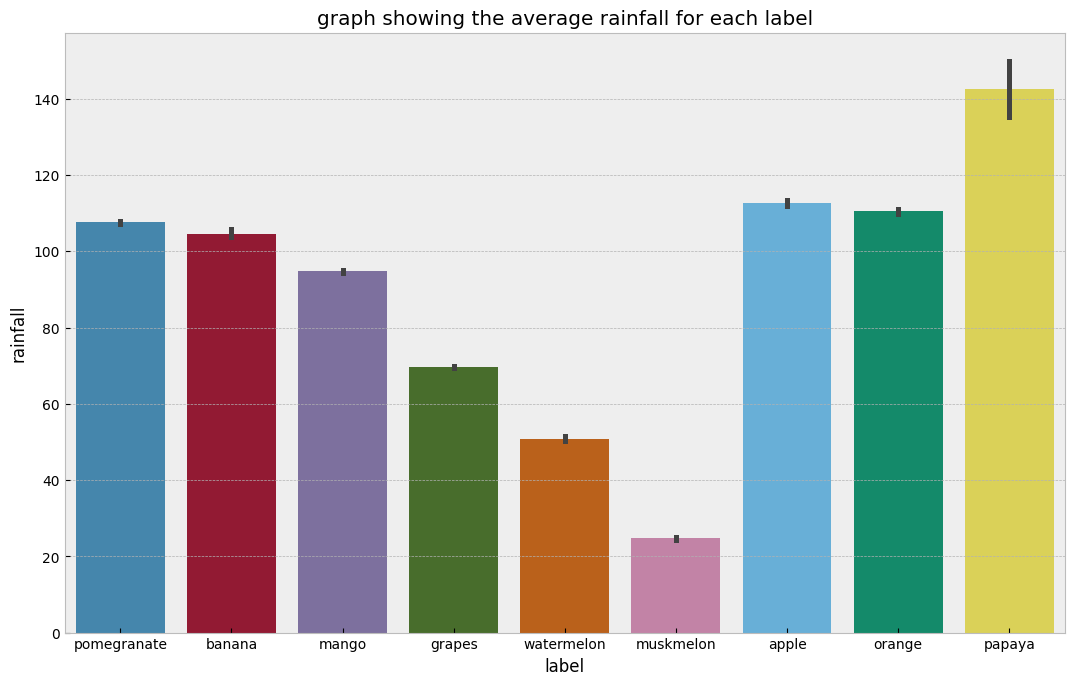
\includegraphics[width=4in,height=2in]{barplot.png}
\caption{Bar Graph}
\label{fig:unevenlight}
\end{figure} 
\subsection{Box Plot}
\begin{lstlisting}[language=Python,basicstyle=\fontsize{9}{11}\selectfont]
fig = plt.figure(figsize=(20,15))
ax=fig.subplots(3,3)
sns.boxplot(x="label",y="N",data=df,ax=ax[0,0])
ax[0,0].set_xticklabels(ax[0,0].get_xticklabels(), rotation=90)

sns.boxplot(x="label",y="P",data=df,ax=ax[0,1])
ax[0,1].set_xticklabels(ax[0,1].get_xticklabels(), rotation=90)

sns.boxplot(x="label",y="K",data=df,ax=ax[0,2])
ax[0,2].set_xticklabels(ax[0,2].get_xticklabels(), rotation=90)

sns.boxplot(x="label",y="temperature",data=df,ax=ax[1,0])
ax[1,0].set_xticklabels(ax[1,0].get_xticklabels(), rotation=90)

sns.boxplot(x="label",y="humidity",data=df,ax=ax[1,1])
ax[1,1].set_xticklabels(ax[1,1].get_xticklabels(), rotation=90)

sns.boxplot(x="label",y="ph",data=df,ax=ax[1,2])
ax[1,2].set_xticklabels(ax[1,2].get_xticklabels(), rotation=90)

sns.boxplot(x="label",y="temperature",data=df,ax=ax[2,0])
ax[2,0].set_xticklabels(ax[2,0].get_xticklabels(), rotation=90)

plt.delaxes(ax[2,1])
plt.delaxes(ax[2,2])
plt.show()
\end{lstlisting}
 
\begin{figure}[h]
\centering
 \footnotesize
 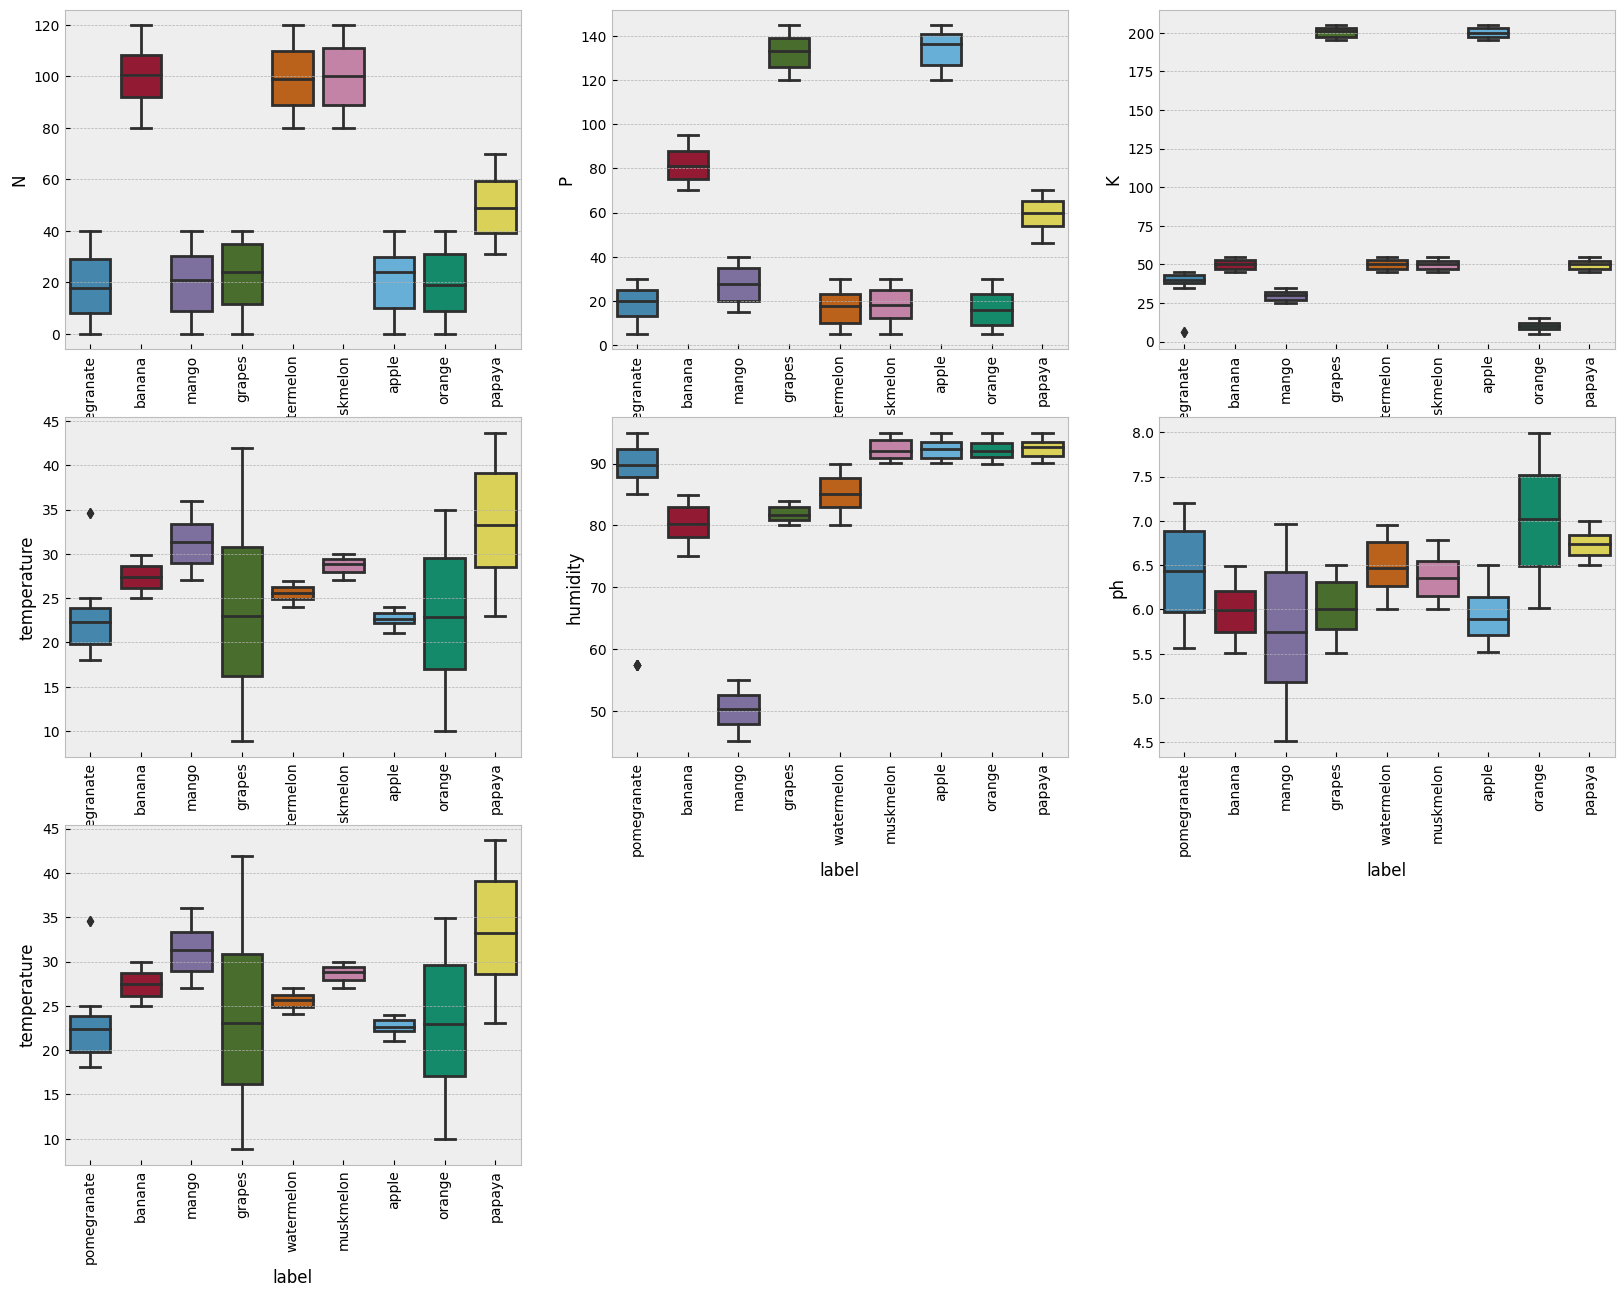
\includegraphics[width=4in,height=2in]{boxplot.png}
\caption{Box Plot}
\label{fig:unevenlight}
\end{figure} 
\subsection{3D Graph}
\begin{lstlisting}[language=Python,basicstyle=\fontsize{9}{11}\selectfont]
data = df.sort_values(["temperature"])
x,y,z=data["temperature"],data["rainfall"],data["humidity"]
fig=plt.figure(figsize=(5,6))
ax2=fig.add_axes([0,0,1,1],projection="3d")
ax2.scatter3D(x,y,z,alpha=0.4)
ax2.set_xlabel("temperature")
ax2.set_ylabel("rainfall")
ax2.set_zlabel("humidity")
plt.show()
ax2.view_init(0,40)
\end{lstlisting}
 
\begin{figure}[h]
\centering
 \footnotesize
 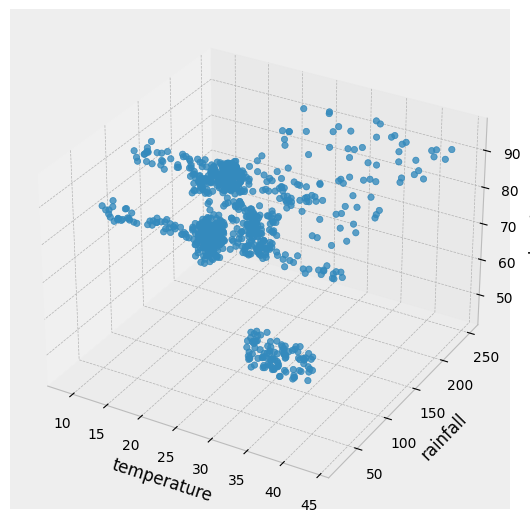
\includegraphics[width=4in,height=4in]{3D graph.png}
\caption{3D Graph}
\label{fig:unevenlight}
\end{figure} 
\vspace{2\baselineskip}
\subsection{Pie Chart}
\begin{lstlisting}[language=Python,basicstyle=\fontsize{9}{11}\selectfont]
explode=[0]*9
explode[0]=0.2
plt.pie(data["rainfall"],shadow=True,explode=explode,labels=data["label"],autopct="%1.0f%%",
textprops={"color":"white"})
plt.legend(bbox_to_anchor=[1,0,0.5,1])
plt.show()
\end{lstlisting}
 
\begin{figure}[h]
\centering
 \footnotesize
 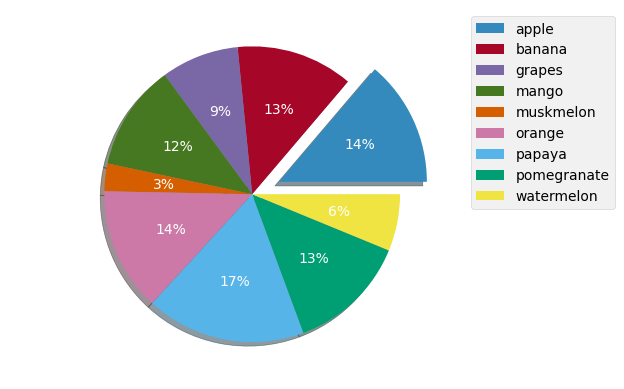
\includegraphics[width=3in,height=2in]{piechart.png}
\caption{Pie Chart}
\label{fig:unevenlight}
\end{figure} 
